% Options for packages loaded elsewhere
\PassOptionsToPackage{unicode}{hyperref}
\PassOptionsToPackage{hyphens}{url}
%
\documentclass[
]{article}
\usepackage{amsmath,amssymb}
\usepackage{lmodern}
\usepackage{iftex}
\ifPDFTeX
  \usepackage[T1]{fontenc}
  \usepackage[utf8]{inputenc}
  \usepackage{textcomp} % provide euro and other symbols
\else % if luatex or xetex
  \usepackage{unicode-math}
  \defaultfontfeatures{Scale=MatchLowercase}
  \defaultfontfeatures[\rmfamily]{Ligatures=TeX,Scale=1}
\fi
% Use upquote if available, for straight quotes in verbatim environments
\IfFileExists{upquote.sty}{\usepackage{upquote}}{}
\IfFileExists{microtype.sty}{% use microtype if available
  \usepackage[]{microtype}
  \UseMicrotypeSet[protrusion]{basicmath} % disable protrusion for tt fonts
}{}
\makeatletter
\@ifundefined{KOMAClassName}{% if non-KOMA class
  \IfFileExists{parskip.sty}{%
    \usepackage{parskip}
  }{% else
    \setlength{\parindent}{0pt}
    \setlength{\parskip}{6pt plus 2pt minus 1pt}}
}{% if KOMA class
  \KOMAoptions{parskip=half}}
\makeatother
\usepackage{xcolor}
\IfFileExists{xurl.sty}{\usepackage{xurl}}{} % add URL line breaks if available
\IfFileExists{bookmark.sty}{\usepackage{bookmark}}{\usepackage{hyperref}}
\hypersetup{
  hidelinks,
  pdfcreator={LaTeX via pandoc}}
\urlstyle{same} % disable monospaced font for URLs
\usepackage{longtable,booktabs,array}
\usepackage{calc} % for calculating minipage widths
% Correct order of tables after \paragraph or \subparagraph
\usepackage{etoolbox}
\makeatletter
\patchcmd\longtable{\par}{\if@noskipsec\mbox{}\fi\par}{}{}
\makeatother
% Allow footnotes in longtable head/foot
\IfFileExists{footnotehyper.sty}{\usepackage{footnotehyper}}{\usepackage{footnote}}
\makesavenoteenv{longtable}
\usepackage{graphicx}
\makeatletter
\def\maxwidth{\ifdim\Gin@nat@width>\linewidth\linewidth\else\Gin@nat@width\fi}
\def\maxheight{\ifdim\Gin@nat@height>\textheight\textheight\else\Gin@nat@height\fi}
\makeatother
% Scale images if necessary, so that they will not overflow the page
% margins by default, and it is still possible to overwrite the defaults
% using explicit options in \includegraphics[width, height, ...]{}
\setkeys{Gin}{width=\maxwidth,height=\maxheight,keepaspectratio}
% Set default figure placement to htbp
\makeatletter
\def\fps@figure{htbp}
\makeatother
\setlength{\emergencystretch}{3em} % prevent overfull lines
\providecommand{\tightlist}{%
  \setlength{\itemsep}{0pt}\setlength{\parskip}{0pt}}
\setcounter{secnumdepth}{-\maxdimen} % remove section numbering
\ifLuaTeX
  \usepackage{selnolig}  % disable illegal ligatures
\fi

\author{}
\date{}

\begin{document}

\hypertarget{model-evaluation-report}{%
\section{Model Evaluation Report}\label{model-evaluation-report}}

\hypertarget{objective}{%
\subsection{Objective}\label{objective}}

This report compares the baseline z-score rule against the logistic
regression classifier on the held-out time-based test split.

\hypertarget{evaluation-setup}{%
\subsection{Evaluation Setup}\label{evaluation-setup}}

\begin{itemize}
\tightlist
\item
  Time split: 60\% train, 20\% validation, 20\% test
\item
  Primary metric: PR-AUC
\item
  Supporting metric: F1 at the validation-selected threshold
\item
  Feature source: \texttt{data/processed/features.parquet}
\end{itemize}

\hypertarget{key-figures}{%
\subsection{Key Figures}\label{key-figures}}

\begin{figure}
\centering
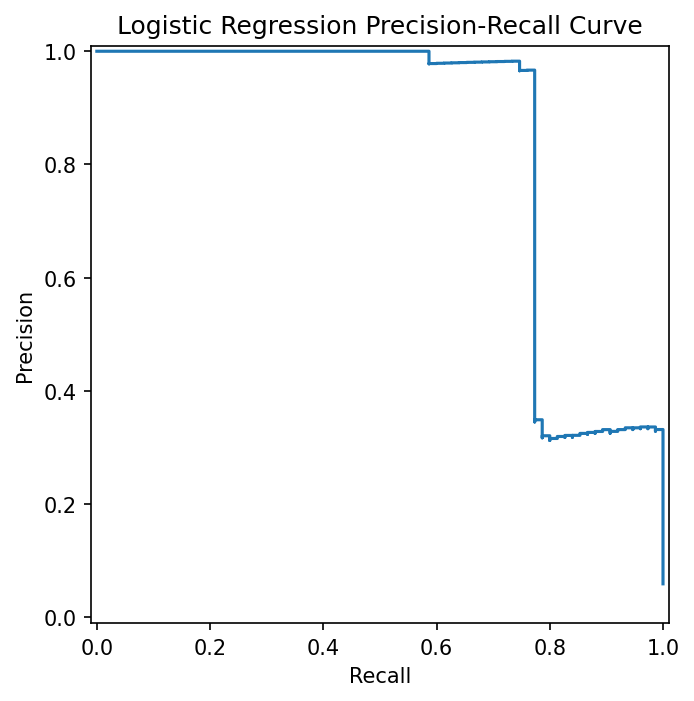
\includegraphics{../img/model_pr_curve.png}
\caption{Precision-Recall Curve}
\end{figure}

\hypertarget{results-summary}{%
\subsection{Results Summary}\label{results-summary}}

The metrics below should be refreshed after each training run and copied
from \texttt{models/artifacts/metrics\_summary.json}.

\begin{longtable}[]{@{}
  >{\raggedright\arraybackslash}p{(\columnwidth - 6\tabcolsep) * \real{0.21}}
  >{\raggedleft\arraybackslash}p{(\columnwidth - 6\tabcolsep) * \real{0.29}}
  >{\raggedleft\arraybackslash}p{(\columnwidth - 6\tabcolsep) * \real{0.29}}
  >{\raggedright\arraybackslash}p{(\columnwidth - 6\tabcolsep) * \real{0.21}}@{}}
\toprule
Model & PR-AUC & F1@Threshold & Notes \\
\midrule
\endhead
Baseline z-score & TBA & TBA & Threshold on standardized realized
volatility \\
Logistic regression & TBA & TBA & Balanced logistic model over
engineered features \\
\bottomrule
\end{longtable}

\hypertarget{interpretation}{%
\subsection{Interpretation}\label{interpretation}}

The main success condition is that the logistic model beats the baseline
on PR-AUC while remaining simple, fast, and easy to explain. If the gain
is marginal, the report should explain whether feature quality, label
sparsity, or market regime instability is the more likely cause.

\hypertarget{artifact-checklist}{%
\subsection{Artifact Checklist}\label{artifact-checklist}}

\begin{itemize}
\tightlist
\item
  Metrics JSON
\item
  Predictions CSV
\item
  Precision-recall curve
\item
  Refreshed Evidently train-vs-test report
\end{itemize}

\end{document}
